% Worked example / template for the solvergraph-diagram skill (upstream PR 2739: per species
% sink accreted dust mass tracking with monofluid TVA dust, if_has_sinks turned into an
% OperationIf). Keep the preamble, the \tikzset styles, the layout patterns (graph-change note,
% top row + OperationIf condition + body frame, columns of (b)) and the legend; replace the
% content. Names, notes and new/modified marks below are specific to this change.
% Styles are in \tikzset so that several tikzpicture pages (one page each) can share them.
% Legend: list exactly the styles used (add removed / modified connection entries when used).
% Build: pdflatex -interaction=nonstopmode <topic>_solvergraph.tex
\documentclass[tikz,border=8pt]{standalone}
\usetikzlibrary{arrows.meta,positioning,fit,backgrounds,calc}

\definecolor{newc}{RGB}{30,140,60}
\definecolor{newfill}{RGB}{225,245,228}
\definecolor{modc}{RGB}{225,120,0}
\definecolor{modfill}{RGB}{255,238,215}
\definecolor{remc}{RGB}{190,40,40}
\definecolor{remfill}{RGB}{250,228,228}
\definecolor{syncfill}{RGB}{225,235,250}
\definecolor{nodefill}{RGB}{245,245,245}

\tikzset{
    every picture/.style={font=\sffamily\small, >={Stealth[length=2.4mm]}},
    % solver graph nodes
    gnode/.style={draw, thick, fill=nodefill, minimum width=36mm, minimum height=9mm,
      align=center},
    % solver graph edges (data)
    gedge/.style={draw, rounded corners=4pt, fill=white, minimum width=30mm,
      minimum height=6mm, font=\sffamily\footnotesize\ttfamily},
    % scheduler synchronized_data edges
    sedge/.style={gedge, fill=syncfill},
    % anything added by the change
    new/.style={draw=newc, dashed, very thick, fill=newfill},
    % existing thing whose behaviour or interface is changed
    modified/.style={draw=modc, solid, very thick, fill=modfill},
    % anything removed by the change
    removed/.style={draw=remc, dashed, very thick, fill=remfill, text=gray!70!black},
    % execution sequence boxes
    seq/.style={draw, fill=nodefill, minimum width=27mm, minimum height=7mm, align=center,
      font=\sffamily\scriptsize\ttfamily},
    % connections: colour (+ dashes) = diff state, line width = access
    % (read only: thin, read / write: thick)
    ro/.style={->, semithick, gray!70!black},
    rw/.style={<->, line width=2.2pt, gray!70!black},
    ronew/.style={->, semithick, newc, dash pattern=on 4pt off 2pt},
    rwnew/.style={<->, line width=2.2pt, newc, dash pattern=on 4pt off 2pt},
    romodified/.style={->, semithick, modc},
    rwmodified/.style={<->, line width=2.2pt, modc},
    roremoved/.style={->, semithick, remc, dash pattern=on 4pt off 2pt},
    rwremoved/.style={<->, line width=2.2pt, remc, dash pattern=on 4pt off 2pt},
    flow/.style={->, thick},
}

\begin{document}
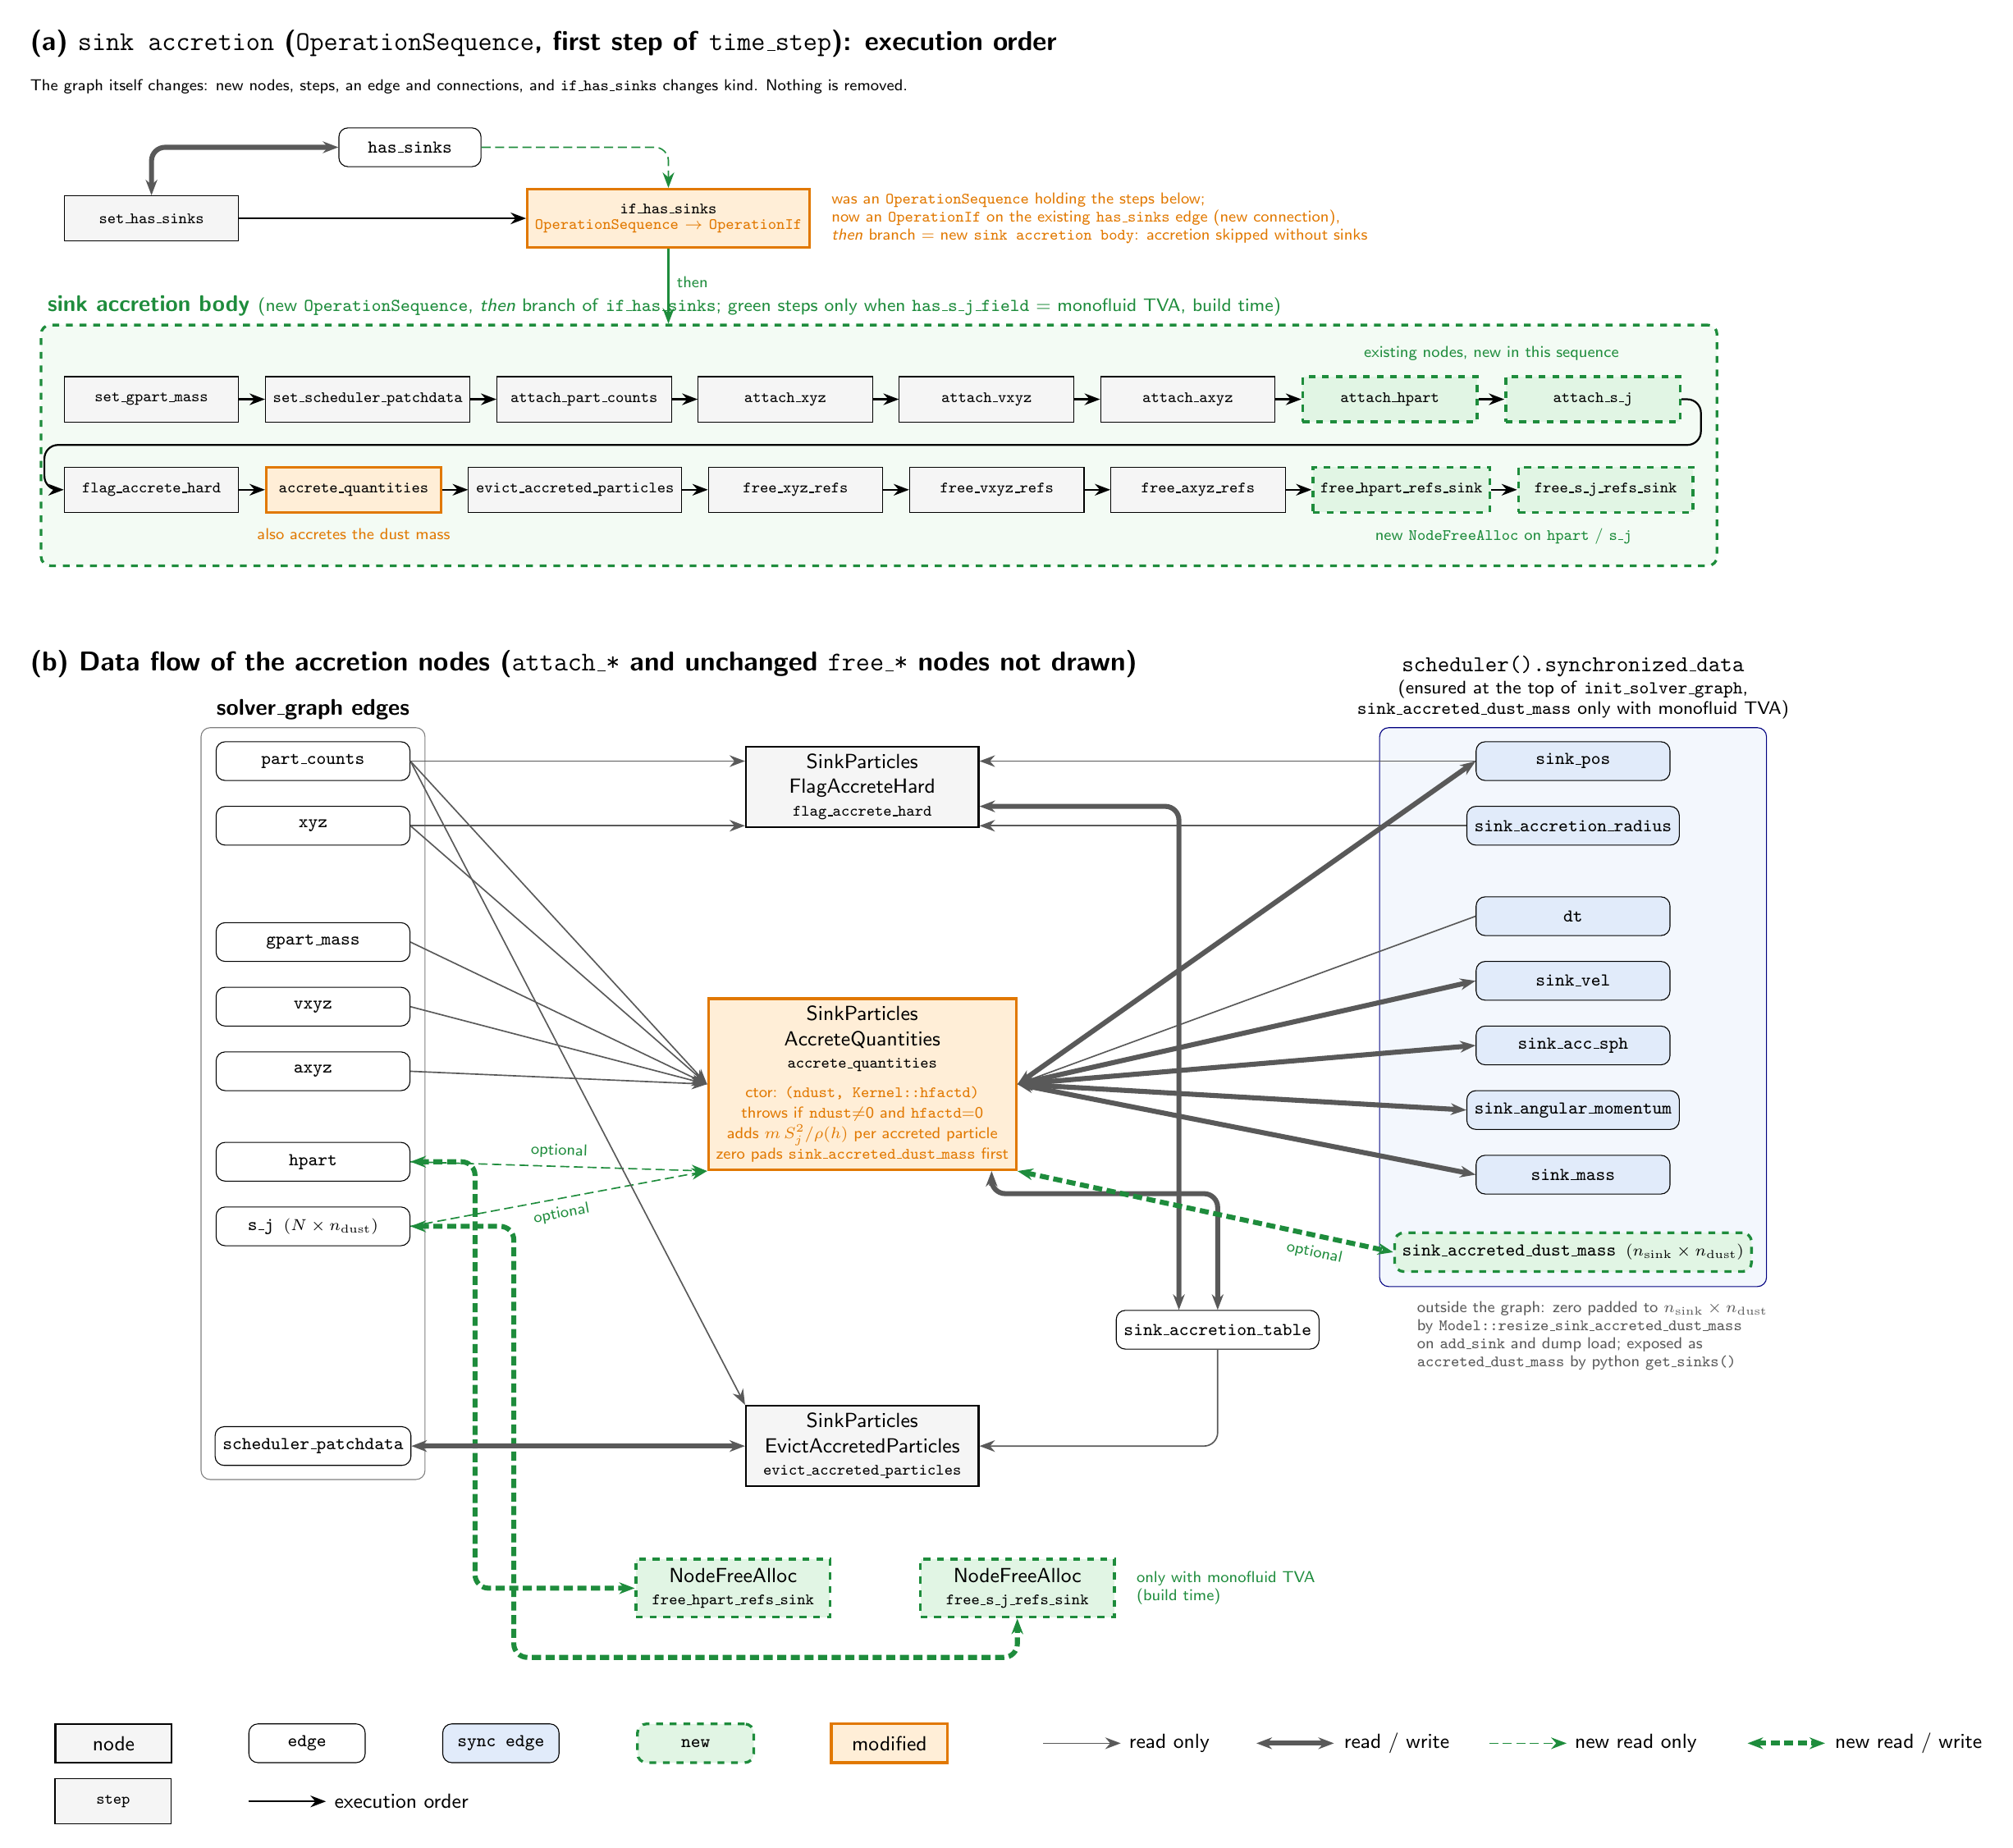
\begin{tikzpicture}

  % ===================================================================================
  % (a) execution order of the "sink accretion" sequence
  % ===================================================================================
  \node[font=\sffamily\bfseries\large, anchor=west] (titleA) at (-2, 10.5)
    {(a) \texttt{sink accretion} (\texttt{OperationSequence}, first step of \texttt{time\_step}): execution order};
  \node[font=\sffamily\scriptsize, anchor=north west, align=left] (graphnote)
    at ($(titleA.south west)+(0,-1mm)$)
    {The graph itself changes: new nodes, steps, an edge and connections,
     and \texttt{if\_has\_sinks} changes kind. Nothing is removed.};

  \begin{scope}[yshift=14mm]
  % --- top level of "sink accretion"
  \node[seq] (t1) at (0, 6.4) {set\_has\_sinks};
  \node[seq, modified, align=center, minimum height=9mm] (t2) at (8, 6.4)
    {if\_has\_sinks\\[-1pt]{\rmfamily\color{modc}\texttt{OperationSequence} $\to$
     \texttt{OperationIf}}};
  \node[gedge, minimum width=22mm] (has_sinks) at (4, 7.5) {has\_sinks};
  \draw[flow] (t1) -- (t2);
  \draw[rw, rounded corners=6pt] (t1.north) |- (has_sinks.west);
  \draw[ronew, rounded corners=6pt] (has_sinks.east) -| (t2.north);
  \node[font=\sffamily\scriptsize, text=modc, anchor=west, align=left]
    at ($(t2.east)+(2mm,0)$)
    {was an \texttt{OperationSequence} holding the steps below;\\
     now an \texttt{OperationIf} on the existing \texttt{has\_sinks} edge (new connection),\\
     \emph{then} branch = new \texttt{sink accretion body}: accretion skipped without sinks};

  % --- body: "sink accretion body" (new OperationSequence, then-branch of if_has_sinks)
  \begin{scope}[node distance=4mm]
    \node[seq] (s1) at (0, 3.6) {set\_gpart\_mass};
    \node[seq, right=of s1] (s2) {set\_scheduler\_patchdata};
    \node[seq, right=of s2] (s3) {attach\_part\_counts};
    \node[seq, right=of s3] (s4) {attach\_xyz};
    \node[seq, right=of s4] (s5) {attach\_vxyz};
    \node[seq, right=of s5] (s6) {attach\_axyz};
    \node[seq, new, right=of s6] (s7) {attach\_hpart};
    \node[seq, new, right=of s7] (s8) {attach\_s\_j};

    \node[seq] (s9) at (0, 2.2) {flag\_accrete\_hard};
    \node[seq, modified, right=of s9] (s10) {accrete\_quantities};
    \node[seq, right=of s10] (s11) {evict\_accreted\_particles};
    \node[seq, right=of s11] (s12) {free\_xyz\_refs};
    \node[seq, right=of s12] (s13) {free\_vxyz\_refs};
    \node[seq, right=of s13] (s14) {free\_axyz\_refs};
    \node[seq, new, right=of s14] (s15) {free\_hpart\_refs\_sink};
    \node[seq, new, right=of s15] (s16) {free\_s\_j\_refs\_sink};
  \end{scope}

  \foreach \a/\b in {s1/s2,s2/s3,s3/s4,s4/s5,s5/s6,s6/s7,s7/s8,
                     s9/s10,s10/s11,s11/s12,s12/s13,s13/s14,s14/s15,s15/s16}
    \draw[flow] (\a) -- (\b);
  % wrap-around arrow from the end of a row to the start of the next one
  \draw[flow, rounded corners=6pt] (s8.east) -- ++(3mm,0) |- ($(s8.south)!0.5!(s9.north)$)
    -| ($(s9.west)+(-3mm,0)$) -- (s9.west);

  \node[font=\sffamily\scriptsize, text=newc, anchor=south, align=center] (n1)
    at ($(s7.north)!0.5!(s8.north)+(0,1mm)$)
    {existing nodes, new in this sequence};
  \node[font=\sffamily\scriptsize, text=newc, anchor=north, align=center] (n2)
    at ($(s15.south)!0.5!(s16.south)+(0,-1mm)$)
    {new \texttt{NodeFreeAlloc} on \texttt{hpart} / \texttt{s\_j}};
  \node[font=\sffamily\scriptsize, text=modc, anchor=north, align=center] (n3)
    at ($(s10.south)+(0,-1mm)$)
    {also accretes the dust mass};

  % frame of the new body sequence
  \begin{scope}[on background layer]
    \node[draw=newc, dashed, very thick, fill=newfill!40, rounded corners, inner xsep=10pt,
      inner ysep=6pt, fit=(s1)(s16)(n1)(n2)(n3),
      label={[font=\sffamily\bfseries, text=newc, anchor=south west]north west:%
        sink accretion body {\mdseries\footnotesize(new \texttt{OperationSequence},
        \emph{then} branch of \texttt{if\_has\_sinks}; green steps only when
        \texttt{has\_s\_j\_field} = monofluid TVA, build time)}}]
      (body) {};
  \end{scope}
  \draw[flow, newc] (t2.south) -- (t2.south |- body.north)
    node[pos=0.45, right, font=\sffamily\scriptsize, text=newc] {then};
  \end{scope}

  % ===================================================================================
  % (b) data flow of the accretion compute nodes
  % ===================================================================================
  \node[font=\sffamily\bfseries\large, anchor=west] (titleB) at (-2, 0.9)
    {(b) Data flow of the accretion nodes (\texttt{attach\_*} and unchanged \texttt{free\_*} nodes not drawn)};

  % --- compute nodes (middle column, in execution order)
  \node[gnode] (flag) at (11, -1.0) {SinkParticles\\FlagAccreteHard\\[-1pt]
    {\scriptsize\ttfamily flag\_accrete\_hard}};
  \node[gnode, modified, minimum height=19mm] (qty) at (11, -5.6)
    {SinkParticles\\AccreteQuantities\\[-1pt]
    {\scriptsize\ttfamily accrete\_quantities}\\[2pt]
    {\scriptsize\color{modc} ctor: \texttt{(ndust, Kernel::hfactd)}}\\[-2pt]
    {\scriptsize\color{modc} throws if \texttt{ndust}$\neq$0 and \texttt{hfactd}=0}\\[-2pt]
    {\scriptsize\color{modc} adds $m\,S_j^2/\rho(h)$ per accreted particle}\\[-2pt]
    {\scriptsize\color{modc} zero pads \texttt{sink\_accreted\_dust\_mass} first}};
  \node[gnode] (evict) at (11, -11.2) {SinkParticles\\EvictAccretedParticles\\[-1pt]
    {\scriptsize\ttfamily evict\_accreted\_particles}};

  \node[gnode, new, minimum width=30mm] (free_h) at (9.0, -13.4) {NodeFreeAlloc\\[-1pt]
    {\scriptsize\ttfamily free\_hpart\_refs\_sink}};
  \node[gnode, new, minimum width=30mm] (free_sj) at (13.4, -13.4) {NodeFreeAlloc\\[-1pt]
    {\scriptsize\ttfamily free\_s\_j\_refs\_sink}};
  \node[font=\sffamily\scriptsize, text=newc, anchor=west, align=left]
    at ($(free_sj.east)+(2mm,0)$) {only with monofluid TVA\\(build time)};

  % --- solver graph edges, inputs (left column)
  \node[gedge] (part_counts) at (2.5, -0.6) {part\_counts};
  \node[gedge] (xyz)         at (2.5, -1.6) {xyz};
  \node[gedge] (gpart_mass)  at (2.5, -3.4) {gpart\_mass};
  \node[gedge] (vxyz)        at (2.5, -4.4) {vxyz};
  \node[gedge] (axyz)        at (2.5, -5.4) {axyz};
  \node[gedge] (hpart)       at (2.5, -6.8) {hpart};
  \node[gedge] (s_j)         at (2.5, -7.8)
    {s\_j {\rm\scriptsize($N\times n_{\rm dust}$)}};
  \node[gedge] (pdat)        at (2.5, -11.2) {scheduler\_patchdata};

  % --- solver graph edge produced by a node of the figure (between the columns)
  \node[gedge] (acc_table) at (16.5, -9.4) {sink\_accretion\_table};

  % --- scheduler synchronized_data edges (right column)
  \node[sedge] (sink_pos)  at (22, -0.6)  {sink\_pos};
  \node[sedge] (sink_racc) at (22, -1.6)  {sink\_accretion\_radius};
  \node[sedge] (dt)        at (22, -3.0)  {dt};
  \node[sedge] (sink_vel)  at (22, -4.0)  {sink\_vel};
  \node[sedge] (sink_acc)  at (22, -5.0)  {sink\_acc\_sph};
  \node[sedge] (sink_l)    at (22, -6.0)  {sink\_angular\_momentum};
  \node[sedge] (sink_mass) at (22, -7.0)  {sink\_mass};
  \node[sedge, new] (sink_dust_mass) at (22, -8.2)
    {sink\_accreted\_dust\_mass {\rm\scriptsize($n_{\rm sink}\times n_{\rm dust}$)}};

  % --- group frames
  \begin{scope}[on background layer]
    \node[draw=gray, rounded corners, inner sep=6pt, fit=(part_counts)(pdat)(s_j),
      label={[font=\sffamily\bfseries]above:solver\_graph edges}] (gl) {};
    \node[draw=blue!50!black, rounded corners, inner sep=6pt, fill=syncfill!40,
      fit=(sink_pos)(sink_dust_mass),
      label={[font=\sffamily\bfseries, align=center]above:%
        \texttt{scheduler().synchronized\_data}\\[-2pt]%
        {\footnotesize\mdseries(ensured at the top of \texttt{init\_solver\_graph},}\\[-3pt]%
        {\footnotesize\mdseries\texttt{sink\_accreted\_dust\_mass} only with monofluid TVA)}}]
      (gs) {};
  \end{scope}
  \node[font=\sffamily\scriptsize, text=gray!70!black, anchor=north, align=left]
    at ($(gs.south)+(3mm,-1mm)$)
    {outside the graph: zero padded to $n_{\rm sink}\times n_{\rm dust}$\\
     by \texttt{Model::resize\_sink\_accreted\_dust\_mass}\\
     on \texttt{add\_sink} and dump load; exposed as\\
     \texttt{accreted\_dust\_mass} by python \texttt{get\_sinks()}};

  % --- flag_accrete_hard
  \draw[ro] (part_counts.east) -- (flag.west |- part_counts.east);
  \draw[ro] (xyz.east) -- (flag.west |- xyz.east);
  \draw[ro] (sink_pos.west) -- (flag.east |- sink_pos.west);
  \draw[ro] (sink_racc.west) -- (flag.east |- sink_racc.west);
  \draw[rw, rounded corners=6pt] (flag.east) ++(0,-0.3) -| ([xshift=-6mm]acc_table.north);

  % --- accrete_quantities (existing connections)
  \draw[ro] (part_counts.east) -- (qty.west);
  \draw[ro] (xyz.east) -- (qty.west);
  \draw[ro] (gpart_mass.east) -- (qty.west);
  \draw[ro] (vxyz.east) -- (qty.west);
  \draw[ro] (axyz.east) -- (qty.west);
  \draw[ro] (dt.west) -- (qty.east);
  \foreach \e in {sink_pos, sink_vel, sink_acc, sink_l, sink_mass}
    \draw[rw] (qty.east) -- (\e.west);
  \draw[rw, rounded corners=6pt] (qty.south east) ++(-0.4,0) |- ++(0,-0.35)
    -| ([xshift=0mm]acc_table.north);

  % --- accrete_quantities (new optional connections, wired only with monofluid TVA)
  \draw[ronew] (hpart.east) -- (qty.south west)
    node[pos=0.5, above, sloped, font=\sffamily\scriptsize, text=newc] {optional};
  \draw[ronew] (s_j.east) -- (qty.south west)
    node[pos=0.5, below, sloped, font=\sffamily\scriptsize, text=newc] {optional};
  \draw[rwnew] (qty.south east) -- (sink_dust_mass.west)
    node[pos=0.8, below, sloped, font=\sffamily\scriptsize, text=newc] {optional};

  % --- new free nodes (rw on the edge they free)
  \draw[rwnew, rounded corners=6pt] (hpart.east) -- ++(1.0,0) |- (free_h.west);
  \draw[rwnew, rounded corners=6pt] (s_j.east) -- ++(1.6,0) |- ($(free_sj.south)+(0,-0.6)$)
    -- (free_sj.south);

  % --- evict_accreted_particles
  \draw[ro] (part_counts.east) -- (evict.north west);
  \draw[ro, rounded corners=6pt] (acc_table.south) |- (evict.east);
  \draw[rw] (pdat.east) -- (evict.west);

  % ===================================================================================
  % legend
  % ===================================================================================
  \begin{scope}[shift={(-1.5,-15.8)}]
    \node[gnode, minimum width=18mm, minimum height=6mm, anchor=west] (l1) at (0,0) {node};
    \node[gedge, minimum width=18mm, anchor=west] (l2) at (3,0) {edge};
    \node[sedge, minimum width=18mm, anchor=west] (l3) at (6,0) {sync edge};
    \node[gedge, new, minimum width=18mm, anchor=west] (l4) at (9,0) {new};
    \node[gnode, modified, minimum width=18mm, minimum height=6mm, anchor=west] (l5)
      at (12,0) {modified};
    \draw[ro] (15.3,0) -- ++(1.2,0) node[right, text=black] {read only};
    \draw[rw] (18.6,0) -- ++(1.2,0) node[right, text=black] {read / write};
    \draw[ronew] (22.2,0) -- ++(1.2,0) node[right, text=black] {new read only};
    \draw[rwnew] (26.2,0) -- ++(1.2,0) node[right, text=black] {new read / write};
    \node[seq, minimum width=18mm, anchor=west] (l6) at (0,-0.9) {step};
    \draw[flow] (3,-0.9) -- ++(1.2,0) node[right, text=black] {execution order};
  \end{scope}

\end{tikzpicture}
\end{document}
